\section{How can I contribute to a project?}

\begin{frame}[fragile,allowframebreaks]{Short answer}

    \begin{figure}
    \centering
    \subfigure{
\includegraphics[width=0.24\textwidth]{assets/GitHub_Logo.png}}\hspace{0.02\textwidth}
    \subfigure{
\includegraphics[width=0.24\textwidth]{assets/Git-Logo-1788C.png}}\hspace{0.02\textwidth}
    \subfigure{
\includegraphics[width=0.26\textwidth]{assets/gitlab-logo-200.png}}
    
    \label{fig:SftwToContribute}
    \end{figure}

\end{frame}

\automateframe{A quick example}{
\begin{itemize}[<+->]
    \item Suppose you want to \textbf{contribute} to a project which is currently working fine
    \item And you want to make a change \textbf{without breaking anything}...
\end{itemize}
}

\begin{frame}{A quick example}
\begin{itemize}
    \item You could use some Cloud Based service and copy your folder and files
\end{itemize}

\begin{figure}
    \centering
    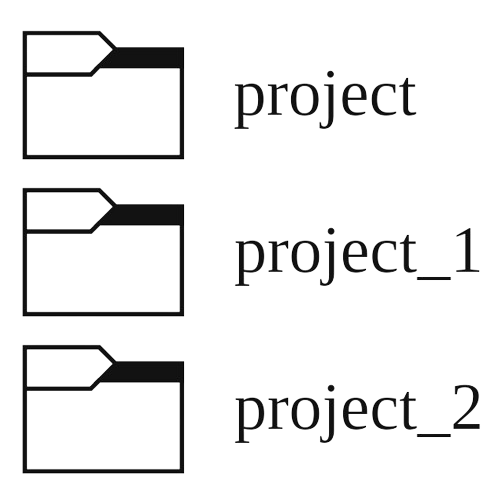
\includegraphics[width=0.35\linewidth]{assets/dir_chaos.png}
    \label{fig:dir_chaos}
\end{figure}

\end{frame}



\begin{frame}{A quick example}
\begin{itemize}
    \item And find yourself with a real mess...
\end{itemize}

\begin{figure}
    \centering
    
\includegraphics[width=0.35\linewidth]{assets/pure_chaos_nobg.png}
    \label{fig:pure_chaos}
\end{figure}

\end{frame}

\begin{frame}{What is git?}
\begin{itemize}
    \item \textbf{Version Control Software} - such as \href{https://help.autodesk.com/view/VAULT/2023/ENU/?guid=GUID-87D9CA09-9881-4506-9465-0677392BCD7E}{Autodesk Vault}
    \end{itemize}
    
\end{frame}

\begin{frame}{What is git?}
How can I actually use it?

\begin{figure}[htbp]
  \begin{minipage}[t]{0.5\textwidth}
    \begin{block}{Code for a Page with an Itemised List}<+->
    \begin{verbatim}
    \begin{frame}{Writing a Simple Slide}
    \framesubtitle{It's really easy!}
        \begin{itemize}[<+->]
            \item A typical slide has bulleted lists
        \item These can be uncovered in sequence
    \end{itemize}\end{frame}
    \end{verbatim}
\end{block}
  \end{minipage}
  \hfill
  \begin{minipage}[t]{0.4\textwidth}
    \centering
    
\includegraphics[width=\linewidth]{assets/gitlab-logo-200.png}
    \caption{Example Image}
    \label{fig:example}
  \end{minipage}
\end{figure}

\vspace{30pt}
Let's give a look to something more practical now...
    
\end{frame}

\automateframe{A practical guide}{
\begin{enumerate}
    \item \href{https://github.com/}{Create a GitHub Account}
    \item 
    \href{https://github.com/firstcontributions/first-contributions}{Search for the first-contributions project}
    \begin{figure}
        \centering
        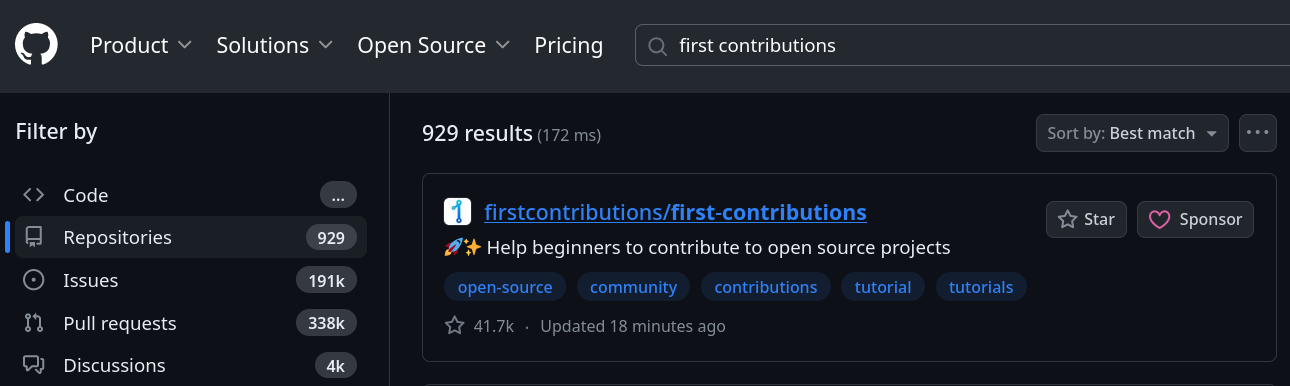
\includegraphics[width=0.75\linewidth]{assets/Screenshot_project.png}
        
        
    \end{figure}
    
    
\end{enumerate}
}

\begin{frame}{A practical guide}
    What are the first files that you should look for in a project?
    \begin{itemize}
    \item \href{https://github.com/firstcontributions/first-contributions/blob/main/README.md}{\textbf{README.md:}}
        \begin{itemize}
            \item Project landing page.
            \item Goals, purpose, how to start, and additional info.
        \end{itemize}
    \end{itemize}

\end{frame}

\begin{frame}{A practical guide}
    What are the first files that you should look for in a project?
    \begin{itemize}
    \item \href{https://github.com/firstcontributions/first-contributions/blob/main/Contributors.md}{\textbf{contributing.md:}}
        \begin{itemize}
            \item Details contributions sought by maintainers.
            \item Process for submitting changes or getting involved.
        \end{itemize}
    \end{itemize}

\end{frame}

\begin{frame}{A practical guide}
    What are the first files that you should look for in a project?
    \begin{itemize}
        \item \href{https://github.com/firstcontributions/first-contributions/blob/main/CODE_OF_CONDUCT.md}{\textbf{Code of Conduct (CoC):}}
        \begin{itemize}
            \item Guidelines for community interaction.
            \item Lists unacceptable behaviors and reporting mechanisms.
            \item Indicates positive behaviors encouraged by maintainers.
        \end{itemize}
    \end{itemize}

\end{frame}

\begin{frame}{A practical guide}
    What are the first files that you should look for in a project?
    \begin{itemize}
            \item 
            \href{https://github.com/firstcontributions/first-contributions/blob/main/LICENSE}{\textbf{license.txt:}}
        \begin{itemize}
            \item Specifies open source license.
            \item Contains full license text.
            \item Essential for understanding usage, modification, and enhancement permissions.
        \end{itemize}
    \end{itemize}

\end{frame}

\begin{frame}{A practical guide}
    \begin{enumerate}
        \item Done
        \item Done
        \item Follow the step by step guide and start contributing
    \end{enumerate}
\end{frame}
